\documentclass[11pt,a4paper]{article}
\usepackage[margin=27mm]{geometry}
\usepackage{fontspec,unicode-math,amsmath,booktabs,graphicx,hyperref}
\setmainfont{STIXGeneral}\setmathfont{STIX Two Math}
\setlength{\parindent}{0pt}\setlength{\parskip}{6pt}
\title{Supported kernels and affine constructions}
\author{Eight-original manuscript comparison}\date{}
\begin{document}\maketitle
\textbf{Written papers.} The eight complete originals contain 246,570 characters. The whole common paper and all eight complete applications contain 176,716 characters. The fixed primary comparison is
\[
 \frac{\sum_i c(S_i)}{c(U)+\sum_i c(A_i)}
 =\frac{246570}{66140+110576}
 =1.395290.
\]
Here $c$ counts nonwhitespace characters after NFC normalization of the accepted selected and calibrated PDF extraction. The primary convention preserves the previously adopted A and Affine coordinate; it was fixed before these factors were evaluated. This measures observed manuscript text, not minimum proof complexity.

All 119 source pages are in scope. The whole 23-page common paper and all 45 application pages are charged, including full tables and references. There is no free common proof from another topic, overlap subtraction or omitted companion. This unifies the eight accepted principal contracts; numerical calculation adds no mathematical, source, question or formalization credit.

\textbf{After acquiring the common theory and required premises.} Conditional factors are $c(S_i)/c(A_i)$ only after acquiring the entire common theory and the actual required computations, presentation data and retained mathematical results. The full local application is charged in every row.
\begin{center}\begin{tabular}{llrrr}\toprule
Original & App & Source & Application & Conditional\\\midrule
L032 & A1 & 16,558 & 8,228 & 2.012397\\
L034 & A2 & 21,433 & 5,801 & 3.694708\\
F016 & A3 & 43,983 & 15,436 & 2.849378\\
F013 & A4 & 25,562 & 6,241 & 4.095818\\
L035 & A5 & 51,019 & 14,514 & 3.515158\\
N009 & A6 & 36,824 & 28,130 & 1.309065\\
L128 & A7 & 18,424 & 8,825 & 2.087705\\
L012 & A8 & 32,767 & 23,401 & 1.400239\\
\bottomrule\end{tabular}\end{center}
The accepted 102 source dispositions and their qualifications remain in force. The scientific source maps are \texttt{scope.json} and \texttt{source\_contract\_map.json}; the input packet's \texttt{source\_scope.json} provides measurement routing. Partial formal scope is separate. These corrected locators clarify the inherited input README without changing any frozen proof or count.
\newpage
\begin{center}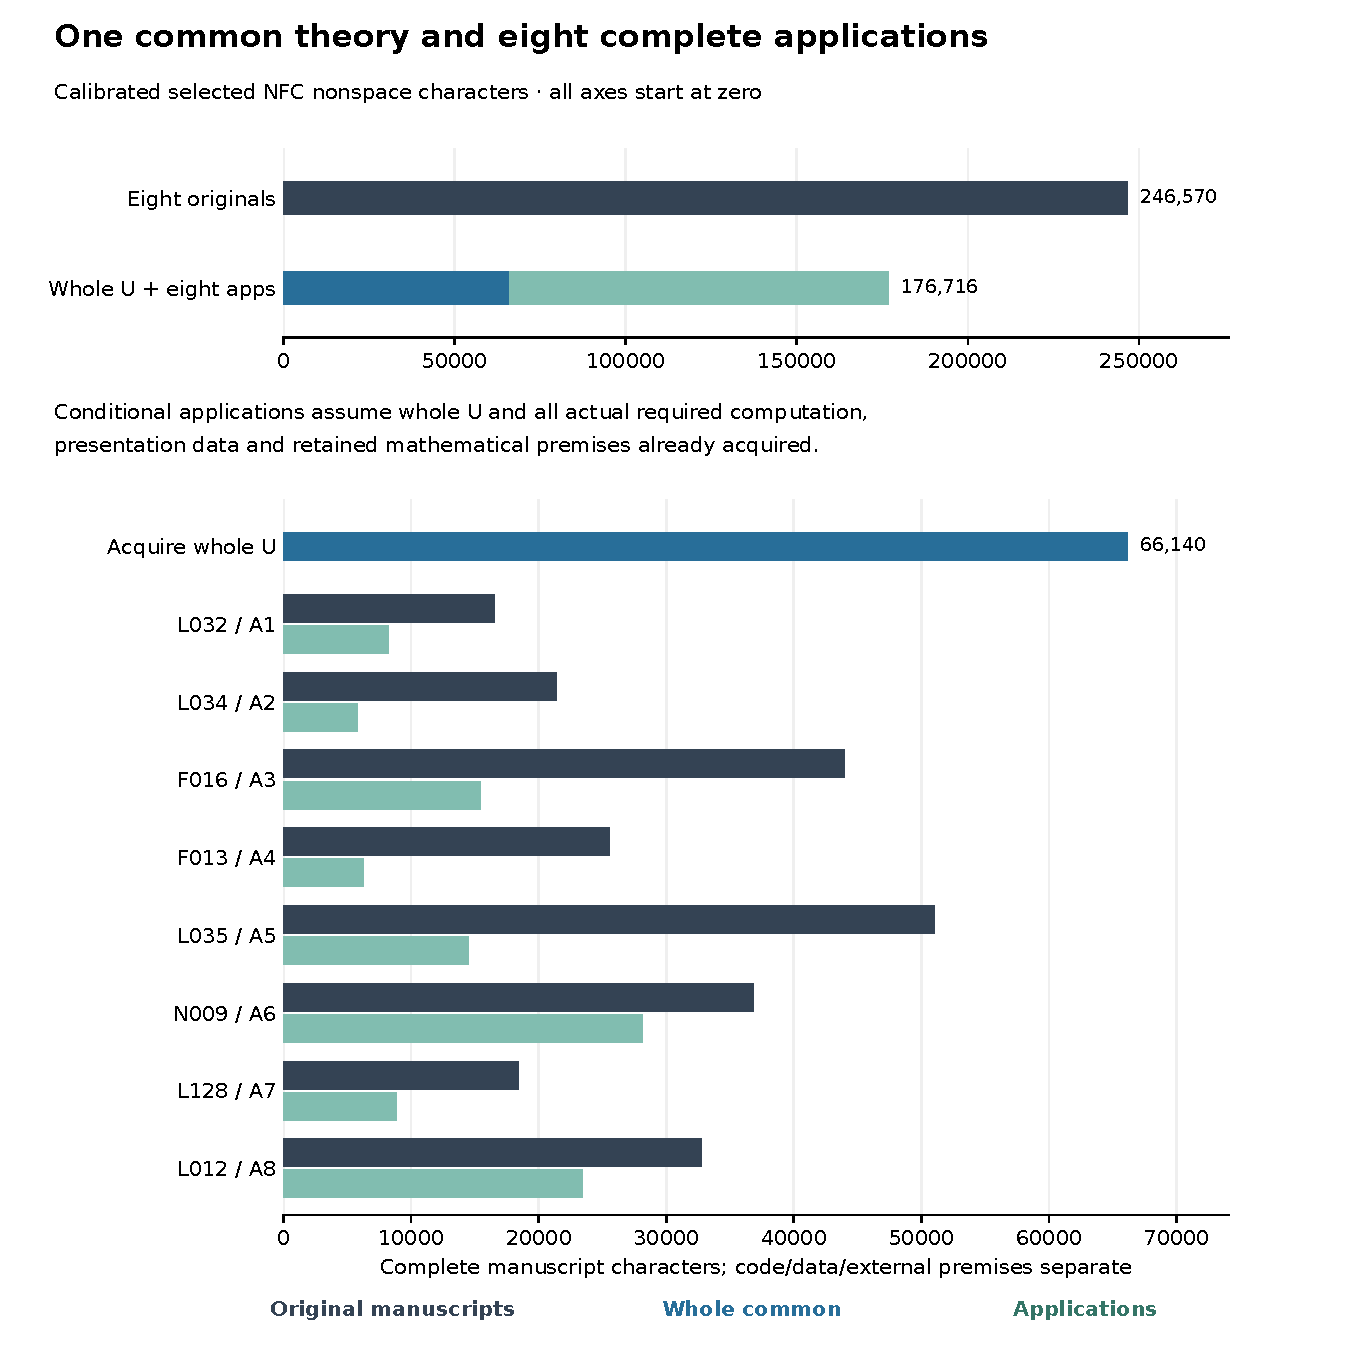
\includegraphics[width=\textwidth]{costs.pdf}\end{center}
The upper graph charges every complete application beside the whole common contribution. The lower graph shows that common acquisition cost and all eight source/application pairs. The 27 bars represent document lengths, not ratios or proof-node counts. All axes start at zero. The source order is documentary; it implies no optimal order or sawtooth claim.

\textbf{Symmetric listing boundary.} Executable programs are excluded from both sides of the manuscript comparison. The accepted source listing screen and replacement TeX inventory retain mathematical proof, algorithm prose, presentations and tables. Required computations remain proof premises even though their code is not part of this written-text factor. Historical source software is unknown, so software-inclusive and optional-validation-inclusive factors are null.
\newpage
\textbf{Complete separate computational inventory.}
\begin{center}\small\begin{tabular}{lrrr}\toprule
Whole files & Count & NFC nonspace chars & Literal bytes\\\midrule
Required computation and data & 11 & 69,489 & 77,369\\
Inherited auxiliary scripts & 3 & 16,581 & 18,741\\
Current operational drivers & 2 & 10,148 & 10,913\\
Partial Lean modules & 14 & 66,657 & 95,292\\
\bottomrule\end{tabular}\end{center}
The three full printed appendices occupy 30 pages. Their primary text costs are 53,035, 17,250 and 1,175 characters. They are alternative representations of the complete computational files, never added to the raw files. The eleven required files include full presentation data and the mathematical replay driver. The two operational drivers remain separate, as do the three inherited auxiliary scripts. Fourteen scoped Lean modules are evidence for limited interfaces, not full formalizations of the source papers.

\textbf{Sensitivity of the whole written factor.}
\begin{center}\small\begin{tabular}{lrrr}\toprule
Unit & Raw & Selected & Calibrated\\\midrule
NFC: Whitespace tokens & 1.620372 & 1.608240 & 1.608266\\
NFC: Alphanumeric units & 1.720264 & 1.705093 & 1.704464\\
NFC: Nonspace characters & 1.408880 & 1.395250 & 1.395290\\
NFC: Collapsed-space characters & 1.446693 & 1.433290 & 1.433327\\
NFC: Collapsed UTF-8 bytes & 1.368923 & 1.356867 & 1.359032\\
NFKC: Whitespace tokens & 1.622816 & 1.610689 & 1.610715\\
NFKC: Alphanumeric units & 1.720264 & 1.705093 & 1.704464\\
NFKC: Nonspace characters & 1.410008 & 1.396385 & 1.396424\\
NFKC: Collapsed-space characters & 1.448042 & 1.434645 & 1.434682\\
NFKC: Collapsed UTF-8 bytes & 1.501664 & 1.488518 & 1.489120\\
\bottomrule\end{tabular}\end{center}
Raw extraction retains running furniture; selected text removes only the exact accepted furniture, and calibration applies the accepted occurrence-bound glyph repairs. All 30 coordinates and 270 exact fractions are preserved in JSON and CSV, with the complete 600 PDF and 300 raw-file input cells unchanged. Printed hyphens and wrap marks remain in measured text. The nine acquisition rows pay the entire common paper first, then complete applications in the displayed source order; required code/data and external costs remain separate.

L035's unextracted image labels on physical pages 9, 10, 12 and 22 remain unmeasured. Full graphics and layout, external classical proofs, installed software/database construction, historical source programs/data and complete formalization costs remain unknown, not zero. The source/font/visual acceptances are reused transparently; this numerical packet performs no source extraction, GAP computation or Lean compilation. Its author worked on earlier proof and audit packets but did not author the unified measurement inputs. A distinct numerical review remains separate.
\end{document}
